\section{数学规划模型}
\subsection{引言}
\subsubsection{多元函数求条件极值}
\begin{align*}
&\max\,\,z=f(x),\quad x=(x_1,x_2,\cdots,x_n)\in R^n \\
&s.t.\quad
    \begin{cases}
        g_i(x)\leq 0,i=1,2,\cdots m
    \end{cases}
\end{align*}
称$x$为决策变量,$f(x)$为目标函数,$g_i\leq 0$为约束条件。
\subsubsection{数学规划模型}
如何分配有限资源,从而达到人们所期望的最优化目标。
\subsubsection{应用}
\begin{itemize}
\item 合理的组合投资
\item 机械制造
\end{itemize}
\subsubsection{赛题}
\begin{itemize}
\item 2002年A题:车灯线光源的设计。
\item 2002年B题:彩票中的数学。
\item 2005年B题:DVD的在线租赁。
\end{itemize}
\subsubsection{建立模型的三要素}
\begin{enumerate}[(1)]
\item 决策变量和参数
    \begin{itemize}
    \item 决策变量---从模型中去寻找
    \item 参数---确定的或者随机的
    \end{itemize}
\item 约束条件
    \begin{itemize}
    \item 由客观的物质条件限制
    \end{itemize}
\item 目标函数(模型中的追求目标)
\end{enumerate}
\subsubsection{模型的分类}
\begin{enumerate}
\item 线性规划问题(目标函数与约束条件全都是线性函数)
\item 整数线性规划问题与0-1线性规划问题
\item 非线性规划问题
\end{enumerate}
\subsubsection{可行解、最优解、次优解以及可行集}
\begin{table}[H]
\begin{tabular}{lll}
\hline
概念 & 说明 &  \\ \hline
可行解 & 满足约束条件的解 &  \\
最优解 & 取得目标函数最优时的可行解 &  \\
次优解 & 比较满意的可行解 &  \\
可行集 & 所有可行解的几何。 &  \\ \hline
\end{tabular}
\caption{概念说明}
\end{table}
\subsection{线性规划}
\begin{example}
某工厂,每日生产8小时,产量不低于1800件/天,但是质量参差不齐。
为把控产品质量,需聘请多名质检员。\par
一级质检员:25件/时,正确率为98\%,工资为4元/时。\par
二级质检员:15件/时,正确率为95\%,工资为3元/时。\par
而质检员出错一件,工厂损失2元。\par
问题,当使质检费最少,应聘请多少一级质检员与二级质检员。
\end{example}
{\heiti 解:}\par
设聘请$x_1$名一级质检员与$x_2$名二级质检员。
\begin{equation*}
z=8*4x_1+8*3x_2+2(8*25*2\%x_1+8*15*5\%x_2)
\end{equation*}
化简可以得出如下的形式:
\begin{align*}
& \min\quad z=40x_1+36x_2 \\
& s.t.\quad
    \begin{cases}
    8*25*x_1+8*15*x_2\geq 1800 \\
    8*25*x_1\leq 1800 \\
    8*15*x_2\leq 1800
    \end{cases}
\end{align*}

\begin{example}
Chebyslev近似:
\begin{equation*}
a_{i1}x_1+a_{i2}x_2+\cdots a_{in}x_n=b_i,\quad (i=1,2,\cdots m)
\end{equation*}
其中$m>>n$,求状态方程组的近似解,使误差尽量地小。
\end{example}
{\heiti 解:}\par
设$\varepsilon_i=b_i-a_{i1}x_1-a_{i2}x_2-\cdots a_{in}x_n$,令$\mu =\max\left\{|\varepsilon_i|,i=1,2,\cdots,n\right\}$
问题转化为求$x_i(i=1,2,\cdots,n)$使得$\mu$尽可能地小。\par
为转换为线性规划问题,设$x_0=\mu$,于是有
\begin{align*}
& \min\quad x_0 \\
& s.t.\quad
    \begin{cases}
    x_0+a_{i1}x_1+a_{i2}x_2+\cdots a_{in}x_n\geq b_i \\
    x_0-a_{i1}x_1-a_{i2}x_2-\cdots a_{in}x_n\geq -b_i \\
    x_0 \geq 0
    \end{cases}
\end{align*}
\subsection{求解方法}
\begin{enumerate}
\item 1939年,苏联康托洛维奇“乘数法”
\item 1947年,美国丹齐克提出单纯形法
\item 1958年,GoMory提出求解整数规划的割平面方法
\item 1962年,苏联学者提出的多项式算法
\end{enumerate}
\subsection{非线性规划}
\begin{itemize}
\item 多项式算法
\item NP-hard(MP)
\end{itemize}
\newpage
\section{2011年B题}
\subsection{题目及其附件}
\begin{figure}[h]
\centering
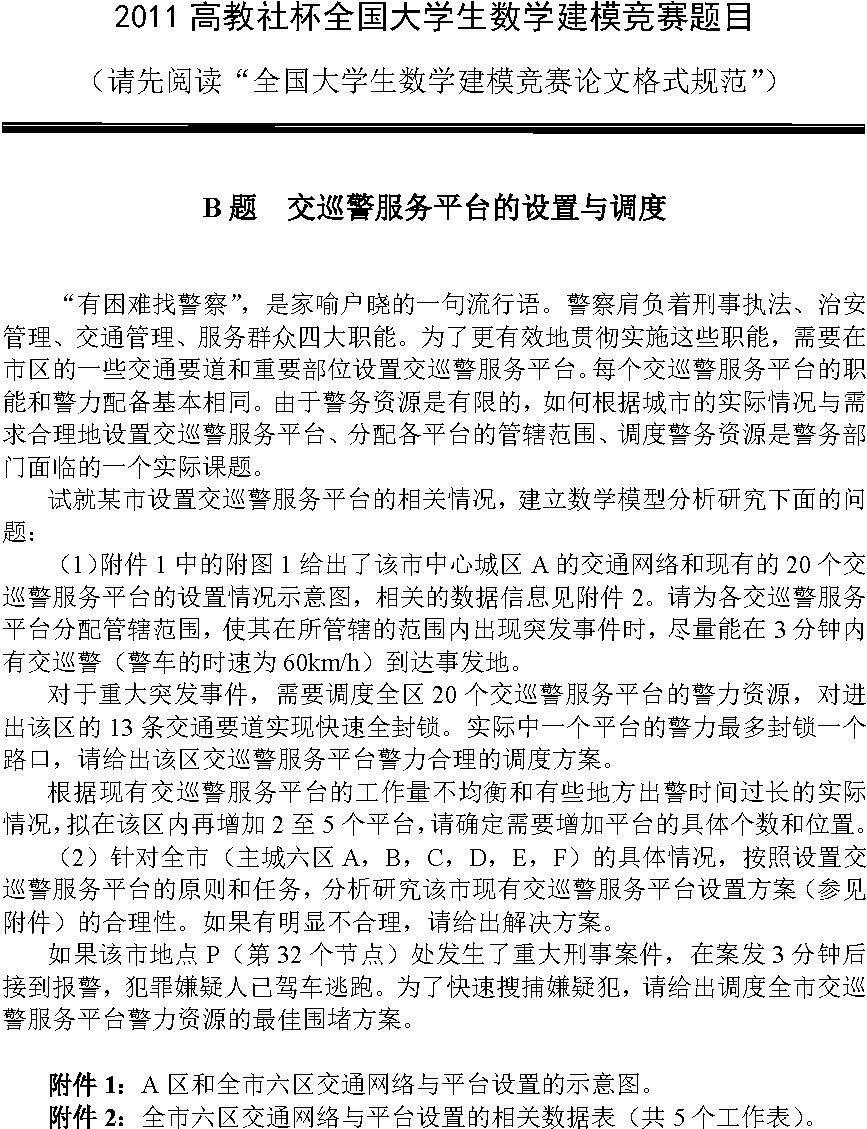
\includegraphics[width=0.72\textwidth]{Figures/2011B_Question}
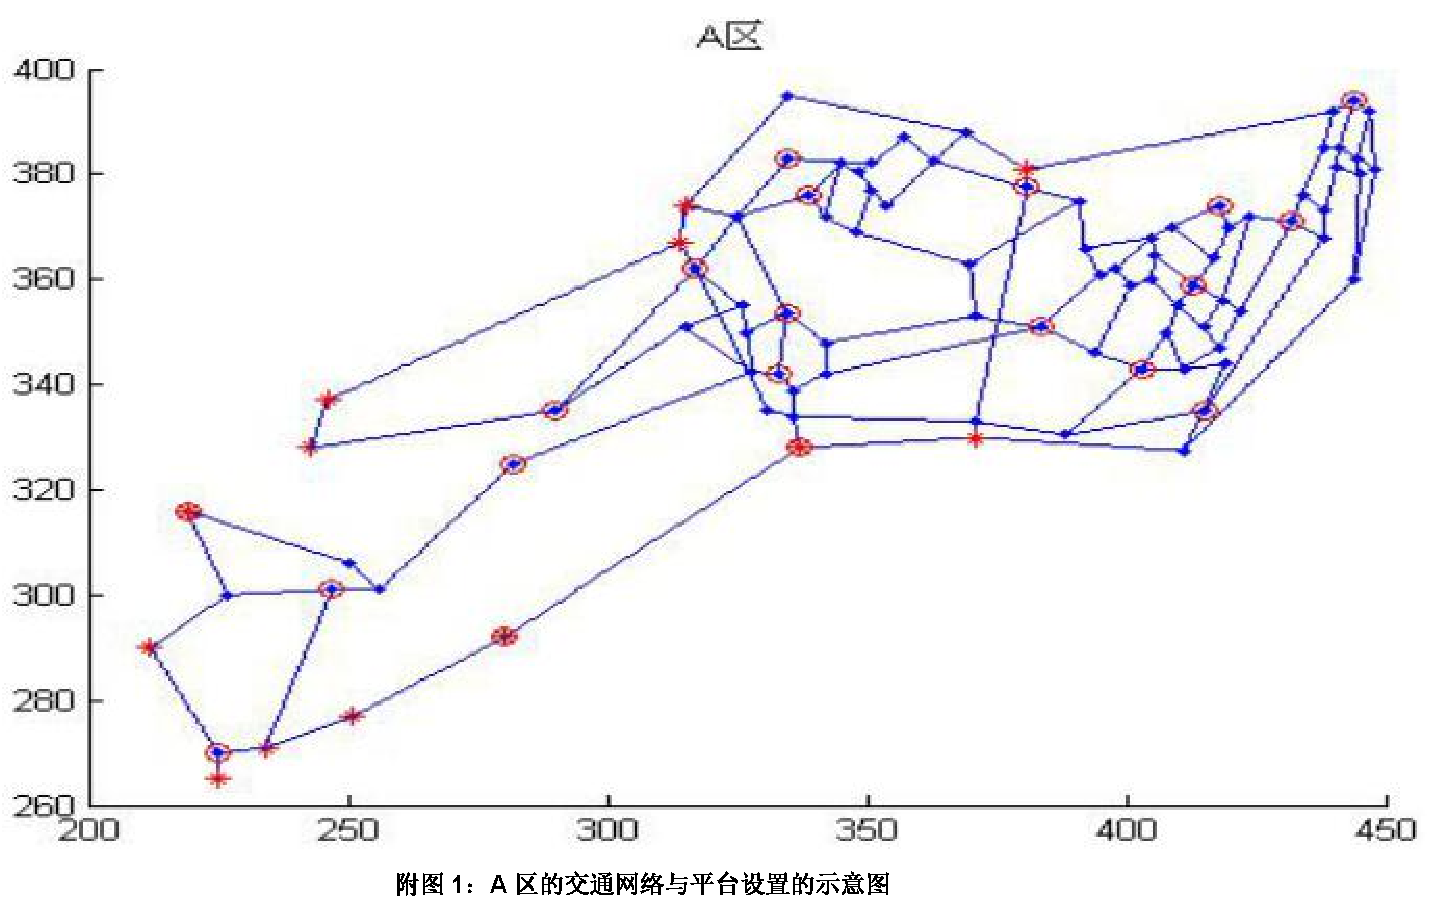
\includegraphics[width=0.45\textwidth,page=1]{Figures/2011B}
\includegraphics[width=0.45\textwidth,page=2]{Figures/2011B}
\end{figure}
\subsection{合理分配A区20个平台管辖范围}
\subsubsection{建立A地区交通网络的赋权图}
\begin{table}[h]
\begin{tabular}{ll}
\hline
符号 & 说明 \\ \hline
$x_i$ & 第$i$个路口,$(i=1,2,\cdots,m)$ \\
$y_j$ & 第$j$个服务平台,$(j=1,2,\cdots,n)$ \\
$L_{ij}$ & 路口$i,j$的连接矩阵 \\
$A_{ij}$ & 路口间的最短路径矩阵,通过$Floyd$计算。 \\
$B_{m\times n}=b_{ij}$ & $x_i$到$y_j$的最短路径 \\ \hline
\end{tabular}
\end{table}
\subsubsection{设置决策变量}
\begin{equation*}
X=(x_{ij})_{m\times n},\quad where\,\,\,x_{ij}\,=\,
\begin{cases}
1, & \text{i地方出事,j出警}\\
0, & \text{i地方出事,j不出警}
\end{cases}
\end{equation*}
\subsubsection{计算出警时间}
\begin{align}
T &=(T_{ij})_{m\times n} \\
T_{ij} &=b_{ij}x_{ij}
\end{align}
\subsubsection{每个警务平台的工作量}
记$G=(g_1,\cdots,g_n)$,其中$g_j$为$y_j$的工作量,$w_i$为$x_i$的案发量。
$$G_i = \sum_{j=1}^{n}x_{ij}\omega_{j}$$
使用矩阵表示:
$$G\,=\,W X\quad where\,\,\,W = (w_1,\cdots,w_m)$$
若记$\bar{G}$为平均工作量,则有
$$\sigma(G)=\sqrt{\frac{1}{n}\sum_{j=1}^{n}(G_j-\bar{G})}$$
\subsubsection{模型的建立}
{\heiti 目标函数}\par
\begin{align*}
\min\quad\max_{\substack{1\leq i\leq m, 1\leq j\leq n}}\quad T_{ij} \\
\min_{X}\quad\sigma(G)
\end{align*}

{\heiti 约束条件}\par
\begin{equation*}
\begin{cases}
\sum_{j=1}^{n}x_{ij}=1,(i=1,2,\cdots,m), &\text{每个路口只有一个平台管理,否则工作重复。} \\
\sum_{i=1}^{m}x_{ij}\geq 1,(j=1,2,\cdots,n), &\text{每个平台至少管理一个路口。} \\
x_{ij}=0\,or\,1, &\text{当i=j时,$x_{ij}=1$}
\end{cases}
\end{equation*}
\subsubsection{模型的求解}
查询MATLAB的优化工具箱,或者使用启发式算法,如蚁群算法,模拟退火算法,遗传算法等。\par
此题为双目标优化,为简化复杂度,可以采用就近原则,削弱目标函数。

\subsection{调动20个平台封锁13个街道}
$D=(d_{ij})_{20\times 13}$,表示A区$y_i$平台到达路口$x_j$的最短路径。
\subsubsection{设置决策变量}
\begin{equation*}
X = (x_{ij})_{20\times 13},\quad where\,\,\,x_{ij}=
\begin{cases}
1, \text{平台$y_i$对路口$x_j$进行封锁} \\
0, \text{不进行封锁}
\end{cases}
\end{equation*}
计算封锁时间
\begin{equation*}
\begin{cases}
T = (T_{ij})_{20\times 13} \\
T_{ij} = d_{ij}x_{ij}
\end{cases}
\end{equation*}
\subsubsection{建立数学模型}
{\heiti 目标函数}\par
$$\min_{X}\quad\max_{\substack{1\leq i\leq 20 \\ 1\leq j\leq 13}}\quad T_{ij}$$

{\heiti 约束条件}\par
\begin{equation*}
\begin{cases}
\sum_{j=1}^{13}x_{ij}\leq 1, &(j=1,2,\cdots,20) \\
\sum_{i=1}^{20}=1, &(i=1,2,\cdots,13) \\
x_{ij}=0 \,or\, 1, &(\text{i=j时,$x_{ij}=1$})\\
\end{cases}
\end{equation*}

\subsection{确定拟增设平台的个数和数目}
通过一个一个加来考虑问题。
\subsubsection{符号说明}
\begin{table}[h]
\begin{tabular}{ll}
\hline
符号 & 说明 \\ \hline
$t_0$ & 增设平台前的最大出警时间 \\
$t_1$ & 增设平台后的最大出警时间 \\
$\sigma_0$ & 增设平台前的工作量的标准差 \\
$\sigma_1$ & 增设平台后的工作量的标准差 \\
$x_{n+1},\cdots,x_{m}$ & 未设置平台的路口 \\ \hline
\end{tabular}
\end{table}
\subsubsection{设置决策变量}
\begin{equation*}
r_j,(r=1,\cdots,m-n),\quad where\,\,\,r_j\,=\,
\begin{cases}
1, & \text{在路口$x_{n+j}$设置平台。} \\
0, & \text{不增设平台。}
\end{cases}
\end{equation*}
\subsubsection{计算设置平台的效益}
$$F\,=\,\rho\frac{t_0-t_1}{t_0}+(1-\rho)\frac{\sigma_0-\sigma_1}{\sigma_0}$$
\subsubsection{模型的建立}
{\heiti 目标函数}\par
\begin{equation*}
\max_{r_j,(j=1,\cdots,m-n)}\quad F
\end{equation*}

{\heiti 约束条件}\par
\begin{equation*}
\begin{cases}
\sum_{i=1}^{m-n}r_i=1 \\
r_i=0 \,or\, 1
\end{cases}
\end{equation*}

\subsection{全市6个区警务平台的设计合理性评价}
如果跨区出警,可将全市看做整体,判断全市警务平台的合理性,从而进行评价\par
如果不跨区出警,分别判断各区警务平台的合理性,从而进行评价。
\subsection{最佳围追堵截方案}
\subsubsection{符号说明}
\begin{table}[h]
\begin{tabular}{ll}
\hline
符号 & 说明 \\ \hline
$D_i, (i=1,\cdots,m)$ & 事发地点的平台到路口$x_i$的最短用时。 \\
$F(t)$ & $\{x_i;D_i\leq t, i=1,\cdots,m\}$ \\
$E(t)$ & $\{F(t)的边界路口位置\}$ \\
$N(t)$ & $\{y_j, x_j\notin F(t), j=1,\cdots,n\}$ \\
$N(E(t)) = P$ & $E(t)$的节点数目 \\ \hline
\end{tabular}
\end{table}
\subsubsection{设置决策变量}
\begin{equation*}
X = (x_{ij})_{P\times n}
x_{ij}=\begin{cases}
1, & \text{平台$y_j$对路口$x_i$进行封锁} \\
0, & \text{反之}
\end{cases}
\end{equation*}
\subsubsection{建立优化模型}
{\heiti 目标函数}\par
\begin{align*}
\min_{X}\quad N(F(t)) \\
\min_{X}\quad\max_{\substack{1\leq i\leq P\\ 1\leq j\leq n}}x_{ij}b_{ij}
\end{align*}

{\heiti 约束条件}\par
\begin{equation*}
\begin{cases}
F(t)\,and\,E(T) & \\
x_{ij}b_{ij} \leq D_i-3 & \text{接到报警有延迟} \\
P=N(E(t)) & \\
\sum_{i=1}^{P}x_{ij}\leq 1, & (j=1,\cdots,n) \\
x_{ij}=0 \,or\, 1 &
\end{cases}
\end{equation*}
\subsubsection{模型的求解}
采用启发式算法,如神经网络式算法。